\RequirePackage{plautopatch}
\documentclass[uplatex,dvipdfmx,a4paper]{jsarticle}
\usepackage{sanzreport}
\title{タイトル}
\author{名前(学籍番号)\thanks{所属}}
\date{\today}
\begin{document}
    \maketitle
    \section{節}
    画像処理によく使われるレナを図~\ref{fig:lena}に示す.
    \begin{figure}[htbp]
        \centering
        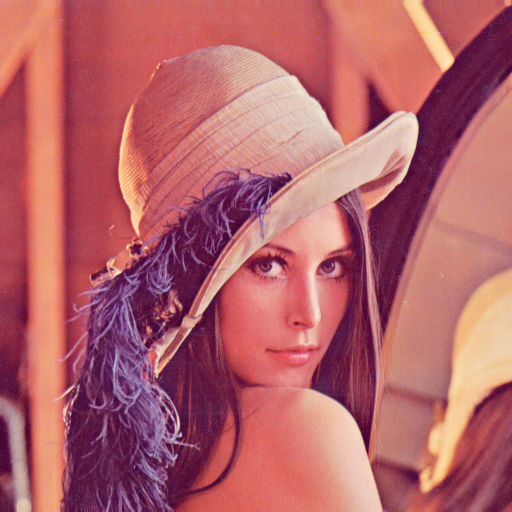
\includegraphics[width=0.3\textwidth]{fig/lena_std}
        \caption{レナ(画像データ)}
        \label{fig:lena}
    \end{figure}
    
    一行の数式は式~\ref{eq:einstein}のように記述する.
    \begin{equation}
        E = mc^2\label{eq:einstein}
    \end{equation}

    表は表~\ref{tab:table}のように記述する.表はジェネレーターで作るのがいい\cite{CreateLa7:online}.
    \begin{table}[htbp]
        \centering
        \caption{工学部でありがちな表}
        \label{tab:table}
        \begin{tabular}{ccc}
        \toprule
        $V_1\si{[V]}$ & $V_2\si{[V]}$ & $a$\\ \midrule
        60 & 30 & 2 \\ 
        120 & 60 & 2 \\ \bottomrule
        \end{tabular}
    \end{table}


    \bibliography{hoge}
    \bibliographystyle{junsrt}
\end{document}